% Alcachofas
\newpage
%\thispagestyle{empty}
\begin{recipe}[source={La mami},
	portion={4 porciones},
	preparationtime={\unit[12]{Minutos}}
	]{Alcachofas}
%	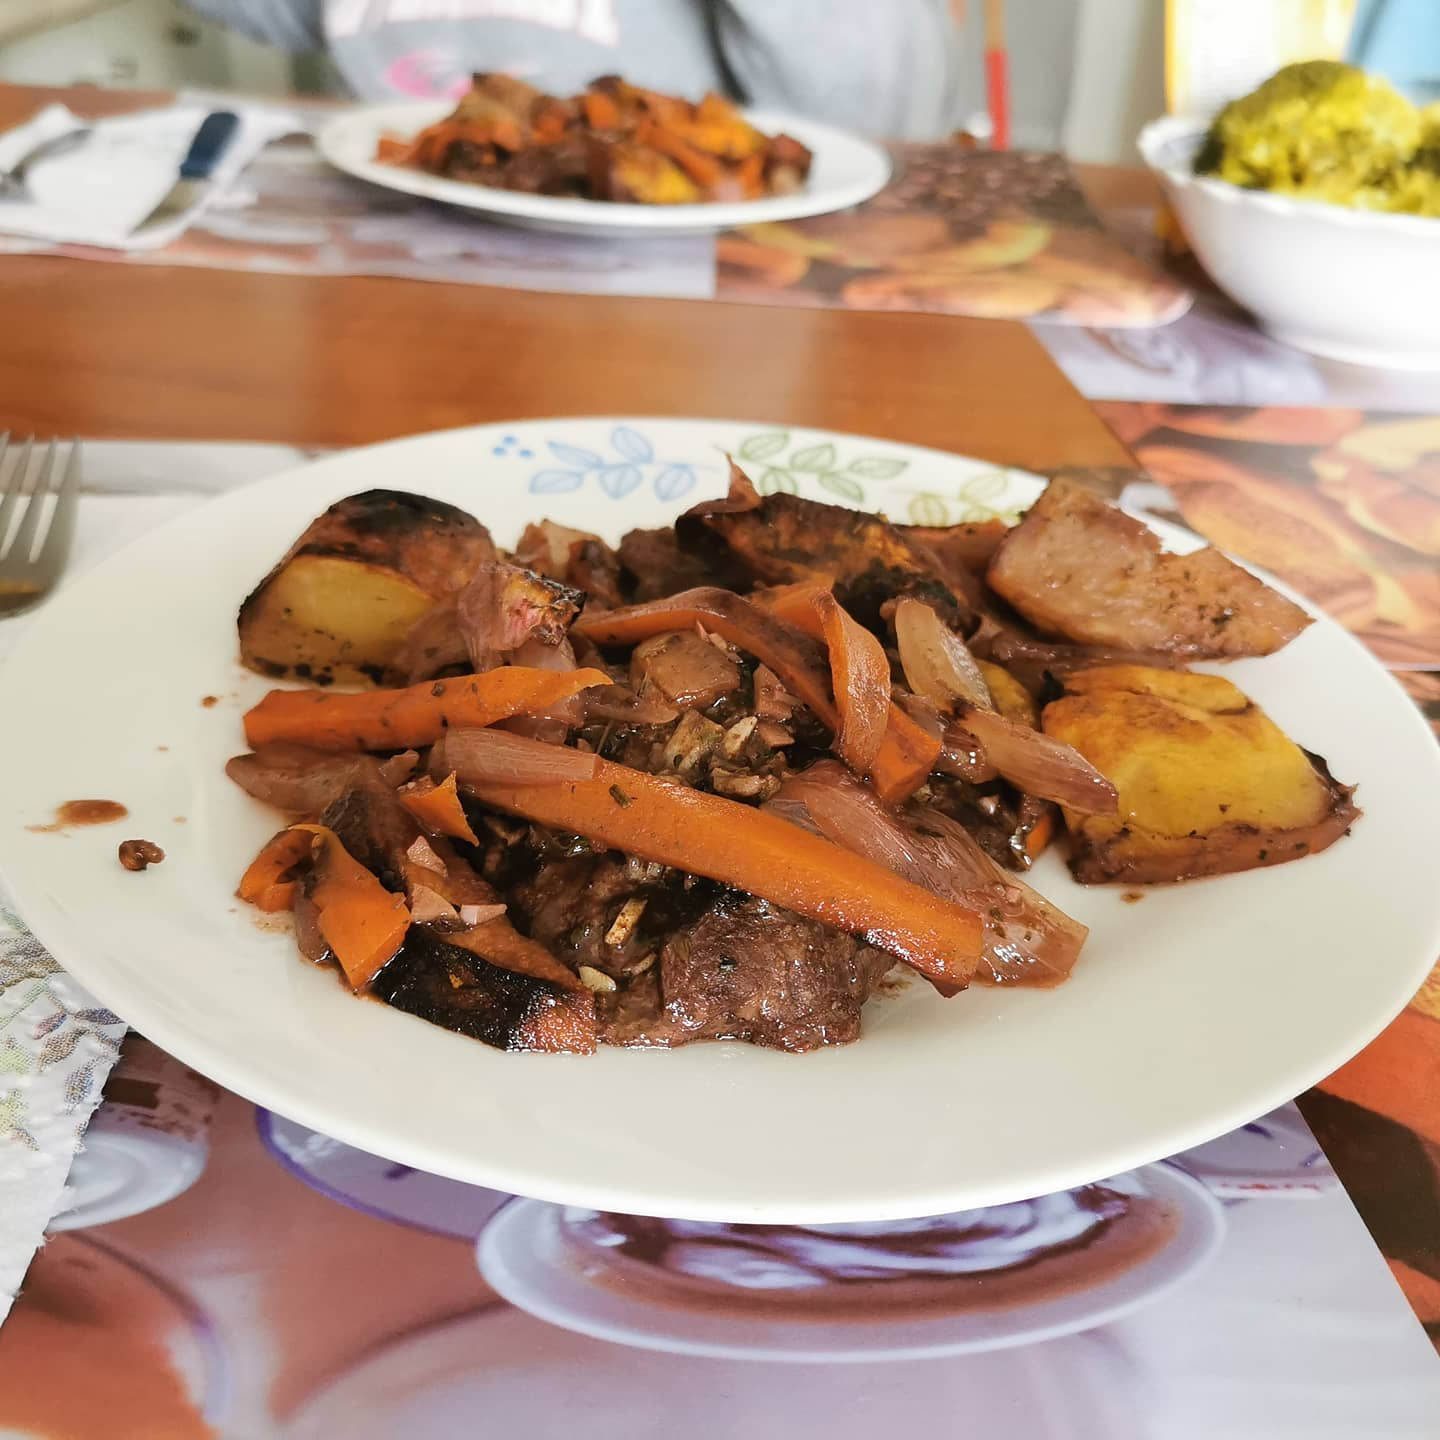
\includegraphics[width=0.25\textwidth]{asado-cacerola}
	\introduction{
		Esta es una receta muy simple de realizar, es típico de las comidas chilenas
	}
	\ingredients{
		4 & alcachofas \\
		$\frac{1}{2}$ & limón \\
		& Para el acompañamiento: \\
		1 & limón \\
		& Aceite de oliva \\
		& Sal \\
		& O en su lugar: \\
		& Vinagre \\
		& Aceite de oliva \\
		& Sal
	}
	\preparation{
		\begin{enumerate}
			\item Lavar muy bien las alcachofas.
			\item En una olla a presión poner agua con una cucharadita de sal y la mitad del limón.
			\item Poner las alcachofas en la olla, cerrar la tapa y cocinar por aproximadamente 12 minutos.
			\item Dejar enfriar, y servir con el acompañamiento.
		\end{enumerate}
	}
	\hint{
		También se puede usar mayonesa en vez del acompañamiento de limón.
	}
\end{recipe}